% --- CAPÍTULO II ---
\chapter{Marco Teórico}

% ===================================================================
% 2.1 ANTECEDENTES
% ===================================================================
\section{Antecedentes teóricos de la investigación}

El seguimiento ocular es una técnica que permite registrar y analizar los movimientos de los ojos, proporcionando información valiosa sobre cómo interactúan los individuos con su entorno visual. Esta tecnología ha sido ampliamente utilizada en diversos campos, como la neurociencia, la psicología, la investigación de la experiencia del usuario y el desarrollo de interfaces hombre-máquina.

La física ha contribuido significativamente a este campo, aportando métodos cuantitativos para el análisis del movimiento ocular. Otras áreas del conocimiento también han desarrollado interés por comprender el fenómeno del movimiento ocular y su aplicación en el desarrollo científico.

A continuación se presentan diversos artículos que constituyen la base teórica de la presente investigación. Estos trabajos sustentan la metodología empleada y las técnicas aplicadas.

\subsection{Eye Aspect Ratio (EAR) para Detección de Somnolencia}

El trabajo de Dewi et al. \cite{dewi2022eye} presenta un método innovador para detectar la somnolencia en conductores en tiempo real, basándose en la métrica conocida como Relación de Aspecto del Ojo (EAR), propuesta originalmente por Soukupová y Čech \cite{soukupova2016real}.

Este estudio de Soukupová y Čech es considerado fundamental en la literatura de visión artificial, ya que marcó un cambio de paradigma en el análisis facial: abandonó el procesamiento intensivo de texturas y píxeles en favor de un modelo puramente geométrico basado en puntos de referencia (\textit{landmarks}). Esta abstracción permitió, por primera vez, ejecutar algoritmos de detección de parpadeo con alta precisión en hardware de recursos limitados (como sistemas embebidos), estableciendo el estándar de eficiencia que domina el campo hasta la actualidad.

La técnica se fundamenta en la identificación de 6 puntos de referencia faciales alrededor del contorno ocular. Matemáticamente, el EAR se calcula mediante la relación entre las distancias verticales y la distancia horizontal del ojo, tal como se expresa en la Ecuación \ref{eq:ear_original}:

\begin{equation}
	EAR = \frac{||p_2 - p_6|| + ||p_3 - p_5||}{2 \cdot ||p_1 - p_4||}
	\label{eq:ear_original}
\end{equation}

Donde $p_1$ y $p_4$ corresponden a las comisuras (extremos horizontales), mientras que los pares $(p_2, p_6)$ y $(p_3, p_5)$ representan los puntos del párpado superior e inferior respectivamente. El numerador calcula el promedio de la apertura vertical, y el denominador normaliza esta medida respecto al ancho del ojo, haciendo la métrica invariante a la escala de la imagen y a la distancia del usuario.

En su estudio aplicado, Dewi et al. \cite{dewi2022eye} concluyen que un umbral de EAR de 0.18 ofrece el mejor compromiso entre precisión y rendimiento. Este método tiene un alto potencial para sistemas de seguridad vial en tiempo real, aunque, como se discutirá en el Capítulo 5, la fórmula original presenta limitaciones de estabilidad ante ruido de alta frecuencia que esta tesis busca mitigar mediante una propuesta geométrica densa.

\subsection{Introduction to Eye Tracking: A Hands-On Tutorial}
Gao et al. \cite{gao2025eye_tracking_tutorial} ofrecen una guía accesible sobre los fundamentos del seguimiento ocular. Combina teoría y práctica para facilitar la comprensión de conceptos clave como el funcionamiento de los dispositivos (cámaras infrarrojas), métricas comunes (fijaciones, sacádicos) y su interpretación en contextos como la interacción humano-computadora.

\subsection{Remote Photoplethysmography}
Allado et al. \cite{allado2022remote} evalúan la precisión de la fotopletismografía remota (rPPG) para medir la frecuencia respiratoria de forma no invasiva utilizando cámaras convencionales. La rPPG demostró una correlación significativa con métodos tradicionales, evitando el uso de sensores físicos.

\subsection{AI in Medical Imaging Technology}
Según estudios recientes \cite{ncbi2023ai}, la inteligencia artificial está transformando la imagen médica. Destacan el uso de redes neuronales convolucionales (CNN) y redes generativas antagónicas (GAN) para mejorar la precisión en la detección de anomalías.

\subsection{Abnormal Ocular Movement in Multiple-System Atrophy}
Zhou et al. \cite{zhou2024abnormal} comparan movimientos oculares en pacientes con atrofia multisistémica y enfermedad de Parkinson. Hallaron que las alteraciones en la velocidad y precisión de los sacádicos voluntarios, así como el nistagmo vertical, son marcadores potenciales para el diagnóstico diferencial.

\subsection{Aplicación de la convolución de matrices}
Giménez et al. \cite{gimenez2016aplicacion} abordan la convolución de matrices como herramienta fundamental en el procesamiento de imágenes. Explican cómo los kernels de convolución permiten aplicar filtros (suavizado, detección de bordes) esenciales para las CNN.

\subsection{Analysis of eye-tracking experiments on Tobii T60}
Weigle et al. \cite{weigle2008analysis} analizan el desempeño del dispositivo Tobii T60. Los resultados muestran que proporciona datos útiles para estudios de visualización, aunque su exactitud puede verse afectada por movimientos de cabeza y condiciones ambientales, sugiriendo la necesidad de una calibración cuidadosa.

La revisión bibliográfica expuesta evidencia el vacío existente en soluciones de bajo costo, nicho que esta investigación pretende ocupar, integrando fundamentos matemáticos, principios físicos y avances computacionales.


% ===================================================================
% 2.2 BASES CONCEPTUALES (Anatomía y Movimientos básicos)
% ===================================================================
\section{Bases conceptuales}

\subsection{Anatomía del Ojo Humano}

El ojo es un órgano que permite percibir la luz, convirtiéndola en señales eléctricas que el cerebro interpreta. Es un sentido clave para la supervivencia humana.

\begin{figure}[h]
	\centering
	\includegraphics[width=0.7\textwidth]{Imagenes/ojo.png}
	\caption{Imagen descriptiva del ojo humano.}
	\label{fig:ojo_anatomia}
\end{figure}

Según Cárdenas \cite{cardenas2024}, las partes principales son:

\begin{description}
	\item[Esclera:] Capa más externa del ojo, de color blanco, formada por tejido conectivo denso.
	\item[Córnea:] Capa transparente frontal que ayuda a enfocar la luz.
	\item[Pupila:] Apertura en el centro del iris que regula la entrada de luz.
	\item[Iris:] Estructura de color que controla el tamaño de la pupila mediante músculos.
	\item[Cristalino:] Lente flexible detrás de la pupila que enfoca la luz en la retina.
	\item[Músculos ciliares:] Rodean al cristalino y modifican su grosor para el enfoque.
	\item[Vítreo:] Sustancia gelatinosa que llena el interior del ojo.
	\item[Retina:] Capa sensible a la luz en la parte posterior que contiene fotorreceptores (conos y bastones).
	\item[Nervio óptico:] Transmite la información visual al cerebro.
\end{description}

\subsection{Movimientos oculares básicos}

El sistema oculomotor permite diversos tipos de movimientos, cada uno con funciones específicas \cite{duchowski2017}:

\subsubsection{Fijaciones}
Son períodos durante los cuales el ojo permanece relativamente estático sobre un punto de interés, permitiendo la adquisición de información visual detallada. Típicamente duran entre 200 y 400 ms.

\subsubsection{Sacádicos}
Movimientos rápidos y balísticos que redirigen la fóvea hacia un nuevo objetivo visual. Son los movimientos más veloces del cuerpo humano, alcanzando velocidades de hasta 900°/s.

\subsubsection{Movimientos de seguimiento suave (Smooth Pursuit)}
Permiten al ojo seguir un objeto en movimiento, manteniendo su imagen en la fóvea. Su velocidad máxima es de aproximadamente 30°/s.

\subsection{La secuencia principal (Main Sequence)}

Bahill et al. \cite{bahill1975} establecieron una relación fundamental conocida como la secuencia principal (\textit{Main Sequence}), que describe la relación matemática y determinista entre la amplitud angular de un movimiento sacádico y su velocidad pico. Esta relación modela el comportamiento balístico del ojo mediante la siguiente expresión exponencial:

\begin{equation}
	V_{\text{max}} = V_{\text{sat}} \left(1 - e^{-A/C}\right)
	\label{eq:bahill}
\end{equation}

donde los parámetros tienen la siguiente interpretación física:
\begin{itemize}
	\item $V_{\text{max}}$ es la velocidad pico alcanzada durante el movimiento (en °/s).
	\item $A$ es la amplitud angular total del desplazamiento (en grados).
	\item $V_{\text{sat}}$ es la velocidad de saturación asintótica ($\approx$ 400-800 °/s en adultos sanos). Este valor representa el límite biomecánico máximo de contracción de los músculos extraoculares.
	\item $C$ es la constante de forma ($\approx$ 10°-20°). Este parámetro define la curvatura de la función y delimita la transición entre movimientos pequeños y grandes.
\end{itemize}

Desde el punto de vista dinámico, esta ecuación revela dos regímenes de comportamiento del sistema oculomotor:
\begin{enumerate}
	\item \textbf{Régimen Lineal (para $A \ll C$):} En movimientos pequeños (microsacadas o sacádicos cortos), la velocidad crece proporcionalmente a la distancia. Esto implica que la duración del movimiento se mantiene casi constante.
	\item \textbf{Régimen de Saturación (para $A \gg C$):} A medida que la amplitud aumenta, la velocidad deja de crecer linealmente y se aproxima asintóticamente a $V_{\text{sat}}$. Esto refleja la incapacidad fisiológica de los músculos para acelerar el globo ocular indefinidamente.
\end{enumerate}

Esta ley neurofisiológica es fundamental no solo para describir la cinemática ocular, sino como herramienta de validación de datos: cualquier trayectoria registrada que se desvíe significativamente de esta curva (puntos muy por encima o muy por debajo) puede ser clasificada automáticamente como un artefacto (ruido instrumental, parpadeo) o como una anomalía motora, garantizando así la autenticidad biológica de la señal procesada.

% ===================================================================
% 2.3 SISTEMA DE CAPTURA Y PROCESAMIENTO
% ===================================================================
\section{Sistema de captura y procesamiento}

\subsection{Tecnologías de seguimiento ocular}

Los sistemas de seguimiento ocular (eye trackers) emplean diversas tecnologías para registrar la posición y el movimiento de los ojos. La mayoría de los dispositivos modernos utilizan cámaras que operan en el espectro infrarrojo cercano (NIR), específicamente entre 850 nm y 940 nm, longitudes de onda imperceptibles para el ojo humano pero que permiten una captura eficiente en diferentes condiciones de iluminación.

\subsubsection{Clasificación según el contacto con el usuario}

\begin{description}
	\item[Dispositivos invasivos:] Requieren contacto directo con el ojo, como lentes de contacto con sensores. Ofrecen alta precisión pero son incómodos y no aptos para uso prolongado.
	
	\item[Dispositivos no invasivos:] Basados en video-oculografía (VOG), utilizan cámaras externas para rastrear características del ojo. Son los más comunes en investigación y aplicaciones comerciales por su balance entre precisión y comodidad.
\end{description}

\subsubsection{Configuraciones de captura}

Los sistemas VOG pueden ser:

\begin{itemize}
	\item \textbf{Montados en cabeza (head-mounted):} Cámaras integradas en gafas o cascos, permitiendo movilidad total del usuario. Ideales para estudios en ambientes naturales.
	
	\item \textbf{Remotos (remote):} Cámaras fijas ubicadas frente al usuario, típicamente integradas en monitores. Requieren que el usuario mantenga la cabeza relativamente estable pero ofrecen mayor comodidad para tareas frente a pantallas.
\end{itemize}

\subsection{Fundamentos de la captura por video}

La captura de imágenes del ojo se basa en principios de óptica geométrica y procesamiento digital de señales. Una cámara digital registra la luz reflejada por el ojo a una tasa de muestreo típica de 60 Hz a 1000 Hz, generando secuencias de fotogramas que son procesados en tiempo real o diferido.

\subsubsection{Características de las cámaras}

Para un sistema de seguimiento ocular efectivo, las cámaras deben cumplir con:

\begin{itemize}
	\item \textbf{Resolución espacial:} Mínimo de 640×480 píxeles para capturar detalles de la pupila y reflexiones corneales.
	
	\item \textbf{Tasa de muestreo temporal:} Al menos 60 Hz para capturar movimientos básicos; 250-1000 Hz para análisis de sacádicos de alta velocidad.
	
	\item \textbf{Rango dinámico:} Capacidad de operar bajo diferentes niveles de iluminación ambiente sin saturación.
	
	\item \textbf{Sincronización:} Los sistemas binoculares requieren sincronización precisa entre cámaras para cálculos estereoscópicos.
\end{itemize}

\subsection{Preprocesamiento de la señal}

Las imágenes capturadas requieren una serie de transformaciones para extraer información útil sobre la posición ocular. Este pipeline de procesamiento incluye:

\subsubsection{Conversión a escala de grises}
La mayoría de algoritmos de seguimiento ocular operan sobre imágenes monocromáticas. La conversión se realiza mediante una combinación ponderada de los canales RGB basada en la percepción luminosa humana:
\begin{equation}
	I = 0.2989R + 0.5870G + 0.1140B
\end{equation}
donde $R$, $G$, $B$ son los componentes de color originales.

\subsubsection{Umbralización global}
Permite segmentar regiones de interés aplicando un umbral $T$. La binarización se define como:
\begin{equation}
	I'(x, y) = \begin{cases} 
		255, & \text{si } I(x, y) > T \\
		0, & \text{si } I(x, y) \leq T 
	\end{cases}
\end{equation}
Esto facilita la detección de bordes de la pupila, que típicamente aparece como la región más oscura de la imagen del ojo.

\subsubsection{Filtro de Savitzky-Golay}

Para el preprocesamiento de las señales oculomotoras, se optó por el filtro digital de Savitzky-Golay en lugar de los métodos tradicionales de promedio móvil. Esta técnica realiza un suavizado basado en el ajuste de mínimos cuadrados locales mediante polinomios de bajo grado dentro de una ventana deslizante. Su operación se describe mediante la convolución discreta:

\begin{equation}
	y[i] = \sum_{k=-M}^{M} c_k x[i+k]
\end{equation}

donde $x[i]$ es la señal original, $y[i]$ la señal suavizada, y $c_k$ son los coeficientes de convolución que dependen del orden del polinomio $p$ y del tamaño de la ventana $2M+1$.

La principal ventaja de este enfoque radica en su capacidad para preservar la forma de la onda (\textit{waveform preservation}). A diferencia de los filtros de media móvil, que actúan como filtros paso bajo agresivos y tienden a atenuar la amplitud de los picos (reduciendo artificialmente la velocidad máxima medida) y ensanchar el ancho temporal de los eventos, el filtro Savitzky-Golay mantiene fielmente los momentos estadísticos de orden superior de la señal. Esto resulta crítico para el análisis de movimientos sacádicos, donde la precisión en la detección de la velocidad pico y la aceleración es prioritaria frente a la simple reducción de ruido estocástico.

\subsubsection{Método de la pupila oscura (Dark Pupil)}
Esta técnica utiliza iluminación infrarroja fuera del eje óptico de la cámara (off-axis illumination). La retina absorbe la luz infrarroja, resultando en una pupila que aparece oscura en la imagen, mientras que la esclera y el iris reflejan la luz. Este alto contraste facilita la segmentación automática de la pupila mediante algoritmos de detección de contornos o ajuste de elipses.

\begin{figure}[h]
	\centering
	\includegraphics[width=0.6\textwidth]{Imagenes/dark_pupil.png}
	\caption{Método de pupila oscura y vector de dirección de la mirada. La pupila aparece como una región oscura debido a la absorción de luz infrarroja por la retina.}
	\label{fig:dark_pupil}
\end{figure}


% ===================================================================
% 2.4 CARACTERIZACIÓN BIOMÉTRICA Y DINÁMICA DE LA SEÑAL
% ===================================================================
\section{Caracterización biométrica y dinámica de la señal}

El análisis moderno de movimientos oculares trasciende la simple ubicación de la mirada (dónde se mira) para enfocarse en la dinámica del movimiento (cómo se mira). Esta investigación se fundamenta en la extracción de características matemáticas avanzadas que describen la complejidad, suavidad y respuesta fisiológica del sistema oculomotor, permitiendo la identificación de patrones únicos por sujeto.

\subsection{Biometría oculomotora}

La biometría oculomotora se basa en la premisa de que los patrones de movimiento ocular son idiosincrásicos; es decir, únicos para cada individuo. Según Komogortsev et al. \cite{komogortsev2010}, esta singularidad surge de la interacción entre dos factores:

\begin{itemize}
	\item \textbf{Factores biomecánicos:} Propiedades anatómicas invariables como la fuerza de los músculos extraoculares, la masa y momento de inercia del globo ocular, la viscosidad de los tejidos orbitales y la elasticidad de los ligamentos suspensorios. Estas características determinan la respuesta mecánica del sistema y son difíciles de replicar entre individuos.
	
	\item \textbf{Factores neurológicos:} Estrategias cognitivas de procesamiento visual, patrones atencionales, y la eficiencia de las vías neuronales que controlan la planificación y ejecución motora. Estos elementos reflejan diferencias en la conectividad cerebral y los procesos de toma de decisiones visuales.
\end{itemize}

A diferencia de biometrías estáticas (como la huella dactilar o el iris), la biometría oculomotora es una biometría comportamental que permite una autenticación continua durante la interacción del usuario con un sistema, sin requerir acciones explícitas de verificación.

\subsection{Pupilometría dinámica y cognitiva}

El diámetro pupilar no responde únicamente a los cambios de iluminación ambiental a través del reflejo fotomotor, sino que presenta fluctuaciones oscilatorias vinculadas directamente a la actividad del Sistema Nervioso Autónomo (SNA). 

Investigaciones clásicas como \cite{beatty1982} establecen que la dilatación pupilar y, particularmente, su velocidad de cambio correlacionan significativamente con:

\begin{itemize}
	\item La carga cognitiva y el esfuerzo mental requerido por una tarea
	\item El estado emocional y niveles de excitación
	\item Procesos de toma de decisiones y resolución de problemas
\end{itemize}

En este estudio, se analiza la velocidad máxima de cambio del diámetro pupilar (\textit{Pupil Velocity}, medida en mm/s) como una métrica de la reactividad del sistema nervioso del individuo. Esta característica temporal, sumada al análisis de la amplitud de las fluctuaciones pupilares, aporta información valiosa para la discriminación entre sujetos, especialmente cuando se combina con características de los movimientos sacádicos.

\subsection{Análisis de la calidad del movimiento: Jerk y suavidad}

Para evaluar la eficiencia y fluidez del control motor ocular, se emplea el concepto físico de \textit{Jerk} (también llamado sobreaceleración o tirón), definido formalmente como la derivada temporal de la aceleración, o equivalentemente, la tercera derivada de la posición respecto al tiempo:

\begin{equation}
	J(t) = \frac{d^3 x(t)}{dt^3} = \frac{da(t)}{dt}
\end{equation}

donde $x(t)$ es la posición angular del ojo en el tiempo $t$, y $a(t)$ es la aceleración.

El sistema nervioso humano optimiza los movimientos voluntarios para minimizar el Jerk, logrando trayectorias suaves y energéticamente eficientes. Un índice elevado de Jerk o una baja suavidad (\textit{smoothness}) en la transición de velocidades durante un sacádico puede indicar:

\begin{itemize}
	\item Fatiga muscular o neurológica
	\item Patologías del sistema oculomotor o cerebeloso
	\item Características motoras específicas de un individuo que no posee un control motor fino
	\item Efectos de sustancias psicoactivas o medicamentos
\end{itemize}

Para cuantificar la suavidad, se utiliza comúnmente el logaritmo de la magnitud adimensional del Jerk (Log Dimensionless Jerk, LDLJ), que permite comparaciones entre movimientos de diferentes amplitudes y duraciones.

\subsection{Análisis de señales no lineales y complejidad fractal}

Los movimientos oculares exhiben comportamientos que no pueden ser descritos completamente por la estadística lineal tradicional (media, varianza, correlación), presentando estructuras caóticas y propiedades fractales que reflejan la complejidad del sistema de control neuromuscular.

Para cuantificar esta complejidad intrínseca, se utiliza la Dimensión Fractal de Higuchi (Higuchi Fractal Dimension, HFD).

Propuesto por Higuchi \cite{higuchi1988}, este algoritmo calcula la rugosidad o complejidad geométrica de una serie temporal sin requerir que la señal sea estacionaria. El método construye múltiples subsecuencias de la señal original con diferentes intervalos de tiempo y calcula la longitud de curva de cada una.

La dimensión fractal resultante ($D_H$) toma valores en el rango [1, 2]:
\begin{itemize}
	\item $D_H \approx 1$: Señal suave y altamente predecible (comportamiento casi lineal)
	\item $D_H \approx 2$: Señal altamente irregular y compleja (similar al ruido browniano)
\end{itemize}

En el contexto de movimientos oculares, la dimensión fractal permite distinguir entre:
\begin{itemize}
	\item Una exploración visual fluida y sistemática (baja dimensión fractal): característica de usuarios con estrategias de búsqueda eficientes y planificadas
	\item Una exploración errática y compleja (alta dimensión fractal): indicativa de búsqueda no estructurada, incertidumbre visual o déficits atencionales
\end{itemize}

Esta métrica captura aspectos de la estrategia cognitiva de búsqueda visual de cada participante que son complementarios a las métricas clásicas de velocidad y precisión.


% ===================================================================
% 2.5 TÉCNICAS DE ANÁLISIS Y CLASIFICACIÓN
% ===================================================================
\section{Técnicas de análisis y clasificación}

Una vez extraídas las características biométricas y dinámicas de las señales oculares, es necesario emplear técnicas estadísticas y de aprendizaje automático para analizar, reducir la dimensionalidad y clasificar los patrones de movimiento ocular con el objetivo de identificar individuos o detectar estados fisiológicos.

\subsection{Estadística descriptiva}

El análisis de los datos oculométricos requiere una caracterización inicial mediante estadística descriptiva. Estas medidas permiten resumir el comportamiento de las variables registradas y evaluar la calidad de la señal adquirida.

\begin{description}
	\item[Media aritmética ($\mu$):] Se utiliza como medida de tendencia central para determinar valores representativos, tales como la duración promedio de una fijación o la velocidad media de un movimiento sacádico. Matemáticamente se define como:
	\begin{equation}
		\mu = \frac{1}{n} \sum_{i=1}^{n} x_i
	\end{equation}
	donde $n$ es el número de observaciones y $x_i$ es cada valor individual.
	
	\item[Desviación estándar ($\sigma$):] Es una métrica fundamental para evaluar la precisión del sistema de seguimiento ocular. En este contexto, la precisión se refiere a la variabilidad o dispersión de los datos adquiridos bajo condiciones repetidas. Se calcula como:
	\begin{equation}
		\sigma = \sqrt{\frac{1}{n} \sum_{i=1}^{n} (x_i - \mu)^2}
	\end{equation}
	Una desviación estándar baja indica alta consistencia entre mediciones repetidas bajo las mismas condiciones, lo cual es indicativo de un sistema estable y confiable. Valores típicos de precisión en sistemas comerciales de seguimiento ocular remoto son de 0.5° a 1° de ángulo visual.
\end{description}

\subsection{Análisis Discriminante Lineal (LDA)}

El Análisis Discriminante Lineal (Linear Discriminant Analysis, LDA) es una técnica estadística de aprendizaje supervisado utilizada para la reducción de dimensionalidad y la clasificación de patrones. Su propósito es proyectar un conjunto de datos de alta dimensión ($d$ características) a un subespacio de menor dimensión ($k$ dimensiones, donde $k < d$), maximizando la separabilidad lineal entre las distintas clases.

A diferencia del Análisis de Componentes Principales (PCA), que es un método no supervisado centrado en maximizar la varianza total de los datos sin considerar las etiquetas de clase, el LDA busca explícitamente modelar la diferencia entre las clases. Para lograr esto, el algoritmo maximiza el Criterio de Fisher, una función objetivo que busca simultáneamente dos metas:

\begin{enumerate}
	\item \textbf{Minimizar la varianza dentro de cada clase} (\textit{within-class scatter}, $S_W$): Asegura que las muestras de una misma clase se agrupen de forma compacta en el espacio proyectado.
	
	\item \textbf{Maximizar la distancia entre las medias de las diferentes clases} (\textit{between-class scatter}, $S_B$): Garantiza que las clases estén lo más separadas posible.
\end{enumerate}

Matemáticamente, el criterio de Fisher se expresa como:
\begin{equation}
	J(w) = \frac{w^T S_B w}{w^T S_W w}
\end{equation}

donde $w$ es el vector de proyección que se busca optimizar.

El resultado es una transformación lineal que preserva la información discriminatoria más relevante, facilitando así la construcción de clasificadores más eficientes y robustos ante la variabilidad de los datos. En el contexto de biometría ocular, el LDA permite reducir un conjunto de decenas de características (velocidades, aceleraciones, dimensiones fractales, etc.) a un espacio de pocas dimensiones donde las diferencias entre sujetos son más evidentes.

\subsection{Máquinas de Vectores de Soporte (SVM)}

Las Máquinas de Vectores de Soporte (Support Vector Machines, SVM) constituyen un conjunto de algoritmos de aprendizaje supervisado desarrollados por Vapnik \cite{vapnik1995}, fundamentados en la teoría del aprendizaje estadístico y la minimización del riesgo estructural. 

El objetivo central de una SVM es encontrar el hiperplano óptimo de separación en un espacio multidimensional. Este hiperplano se elige de tal manera que maximice el margen entre las clases, entendiendo el margen como la distancia geométrica entre la frontera de decisión y los puntos de entrenamiento más cercanos de cada clase, a los cuales se les denomina vectores de soporte.

\subsubsection{Formulación matemática}

Para un problema de clasificación binaria, donde los datos de entrenamiento son $(x_i, y_i)$ con $x_i \in \mathbb{R}^d$ y $y_i \in \{-1, +1\}$, el hiperplano de separación se define como:
\begin{equation}
	w^T x + b = 0
\end{equation}

El problema de optimización busca maximizar el margen, lo cual equivale a minimizar $||w||^2$ sujeto a las restricciones:
\begin{equation}
	y_i(w^T x_i + b) \geq 1, \quad \forall i
\end{equation}

\subsubsection{Kernel RBF para datos no lineales}

Debido a que los datos biométricos y oculares frecuentemente presentan fronteras de decisión complejas y no lineales, este trabajo implementa SVM utilizando el truco del kernel, específicamente la Función de Base Radial (Radial Basis Function, RBF):

\begin{equation}
	K(x_i, x_j) = \exp\left(-\gamma ||x_i - x_j||^2\right)
\end{equation}

donde $\gamma$ es un hiperparámetro que controla la influencia de cada vector de soporte.

Esta técnica matemática permite mapear implícitamente los vectores de entrada originales a un espacio de características de mayor (incluso infinita) dimensión donde las clases se vuelven linealmente separables. Esto dota al modelo de la capacidad para capturar relaciones no lineales complejas en la dinámica ocular sin incurrir en un costo computacional prohibitivo, ya que el cálculo se realiza mediante productos internos en el espacio original a través de la función kernel.

\subsection{Random Forest (Bosque Aleatorio)}
\label{subsec:random_forest}

Random Forest es un algoritmo de aprendizaje conjunto (\textit{ensemble learning}) diseñado para tareas de clasificación y regresión, propuesto originalmente por Breiman \cite{breiman2001}. Su funcionamiento se basa en la construcción de una colección de múltiples clasificadores base, específicamente árboles de decisión, durante la etapa de entrenamiento, para luego combinar sus predicciones mediante votación.

\subsubsection{Principios fundamentales}

La robustez del algoritmo radica en combinar dos técnicas complementarias:

\begin{enumerate}
	\item \textbf{Bagging (Bootstrap Aggregating):} Para construir cada árbol, se genera una muestra de entrenamiento distinta mediante un muestreo con reemplazo (\textit{bootstrap sampling}) del conjunto de datos original. Esto significa que cada árbol se entrena con aproximadamente el 63.2\% de las muestras únicas, mientras que el resto (out-of-bag samples) pueden usarse para validación interna.
	
	\item \textbf{Selección aleatoria de características:} En cada nodo de decisión del árbol, el algoritmo no evalúa todas las $d$ variables posibles para determinar la mejor partición, sino únicamente un subconjunto aleatorio de $\sqrt{d}$ características (para clasificación) o $d/3$ (para regresión). Esta aleatorización fuerza a los árboles a explorar diferentes aspectos de los datos.
\end{enumerate}


\subsubsection{Criterio de Selección de Atributos: Índice de Gini}

Para determinar la división óptima en cada nodo de los árboles que conforman el bosque, el algoritmo utiliza el Índice de Impureza de Gini. Esta métrica mide la probabilidad de clasificar incorrectamente un elemento elegido al azar si se etiquetara de acuerdo con la distribución de clases en el subconjunto de datos.

Matemáticamente, para un nodo dado $t$, el índice de Gini $G(t)$ se define como:
\begin{equation}
	G(t) = 1 - \sum_{i=1}^{C} p(i|t)^2
\end{equation}

Donde:
\begin{itemize}
	\item $C$ es el número total de clases (en este estudio, el número de participantes).
	\item $p(i|t)$ es la probabilidad relativa de la clase $i$ en el nodo $t$.
\end{itemize}

Un índice de Gini igual a 0 indica un nodo puro (todos los elementos pertenecen a la misma clase), mientras que un valor cercano a 1 indica una distribución aleatoria de clases. El algoritmo busca, en cada paso, la característica y el punto de corte que maximicen la reducción de la impureza total, permitiendo así que el modelo aprenda los patrones más discriminativos de las señales oculomotoras.

\subsubsection{Importancia de las Variables (Feature Importance)}

Más allá de la clasificación, el algoritmo de Random Forest permite cuantificar la relevancia de cada métrica extraída (como la velocidad sacádica o la dimensión fractal) mediante la \textit{Importancia de Características por Impureza de Gini}.

Este valor se calcula sumando todas las reducciones del índice de Gini que ocurren cada vez que una variable específica se utiliza para dividir un nodo, promediando dicho valor sobre todos los árboles del bosque. Matemáticamente, la importancia de una característica $X_j$ se define como:

\begin{equation}
	I(X_j) = \frac{1}{T} \sum_{t=1}^{T} \sum_{n \in nodes(t), v(n)=X_j} \Delta G(n)
\end{equation}

Donde:
\begin{itemize}
	\item $T$ es el número total de árboles.
	\item $\Delta G(n)$ es el decremento en la impureza de Gini al realizar la división en el nodo $n$.
	\item $v(n)=X_j$ indica que la variable $X_j$ fue la utilizada para realizar la partición en ese nodo.
\end{itemize}

Aquellas variables que generen nodos más puros (reducciones de Gini más drásticas) de manera consistente en todo el bosque obtendrán una puntuación de importancia mayor. En el contexto de esta tesis, este análisis permite identificar cuáles de los parámetros oculomotores son biométricamente más significativos para distinguir la identidad de un individuo frente a la población de estudio.

\subsubsection{Predicción y ventajas}

La clasificación de una nueva instancia se obtiene mediante votación por mayoría simple de todos los árboles del bosque:
\begin{equation}
	\hat{y} = \text{moda}\{h_1(x), h_2(x), ..., h_T(x)\}
\end{equation}

donde $h_t(x)$ es la predicción del árbol $t$-ésimo y $T$ es el número total de árboles.

\begin{figure}[h]
	\centering
	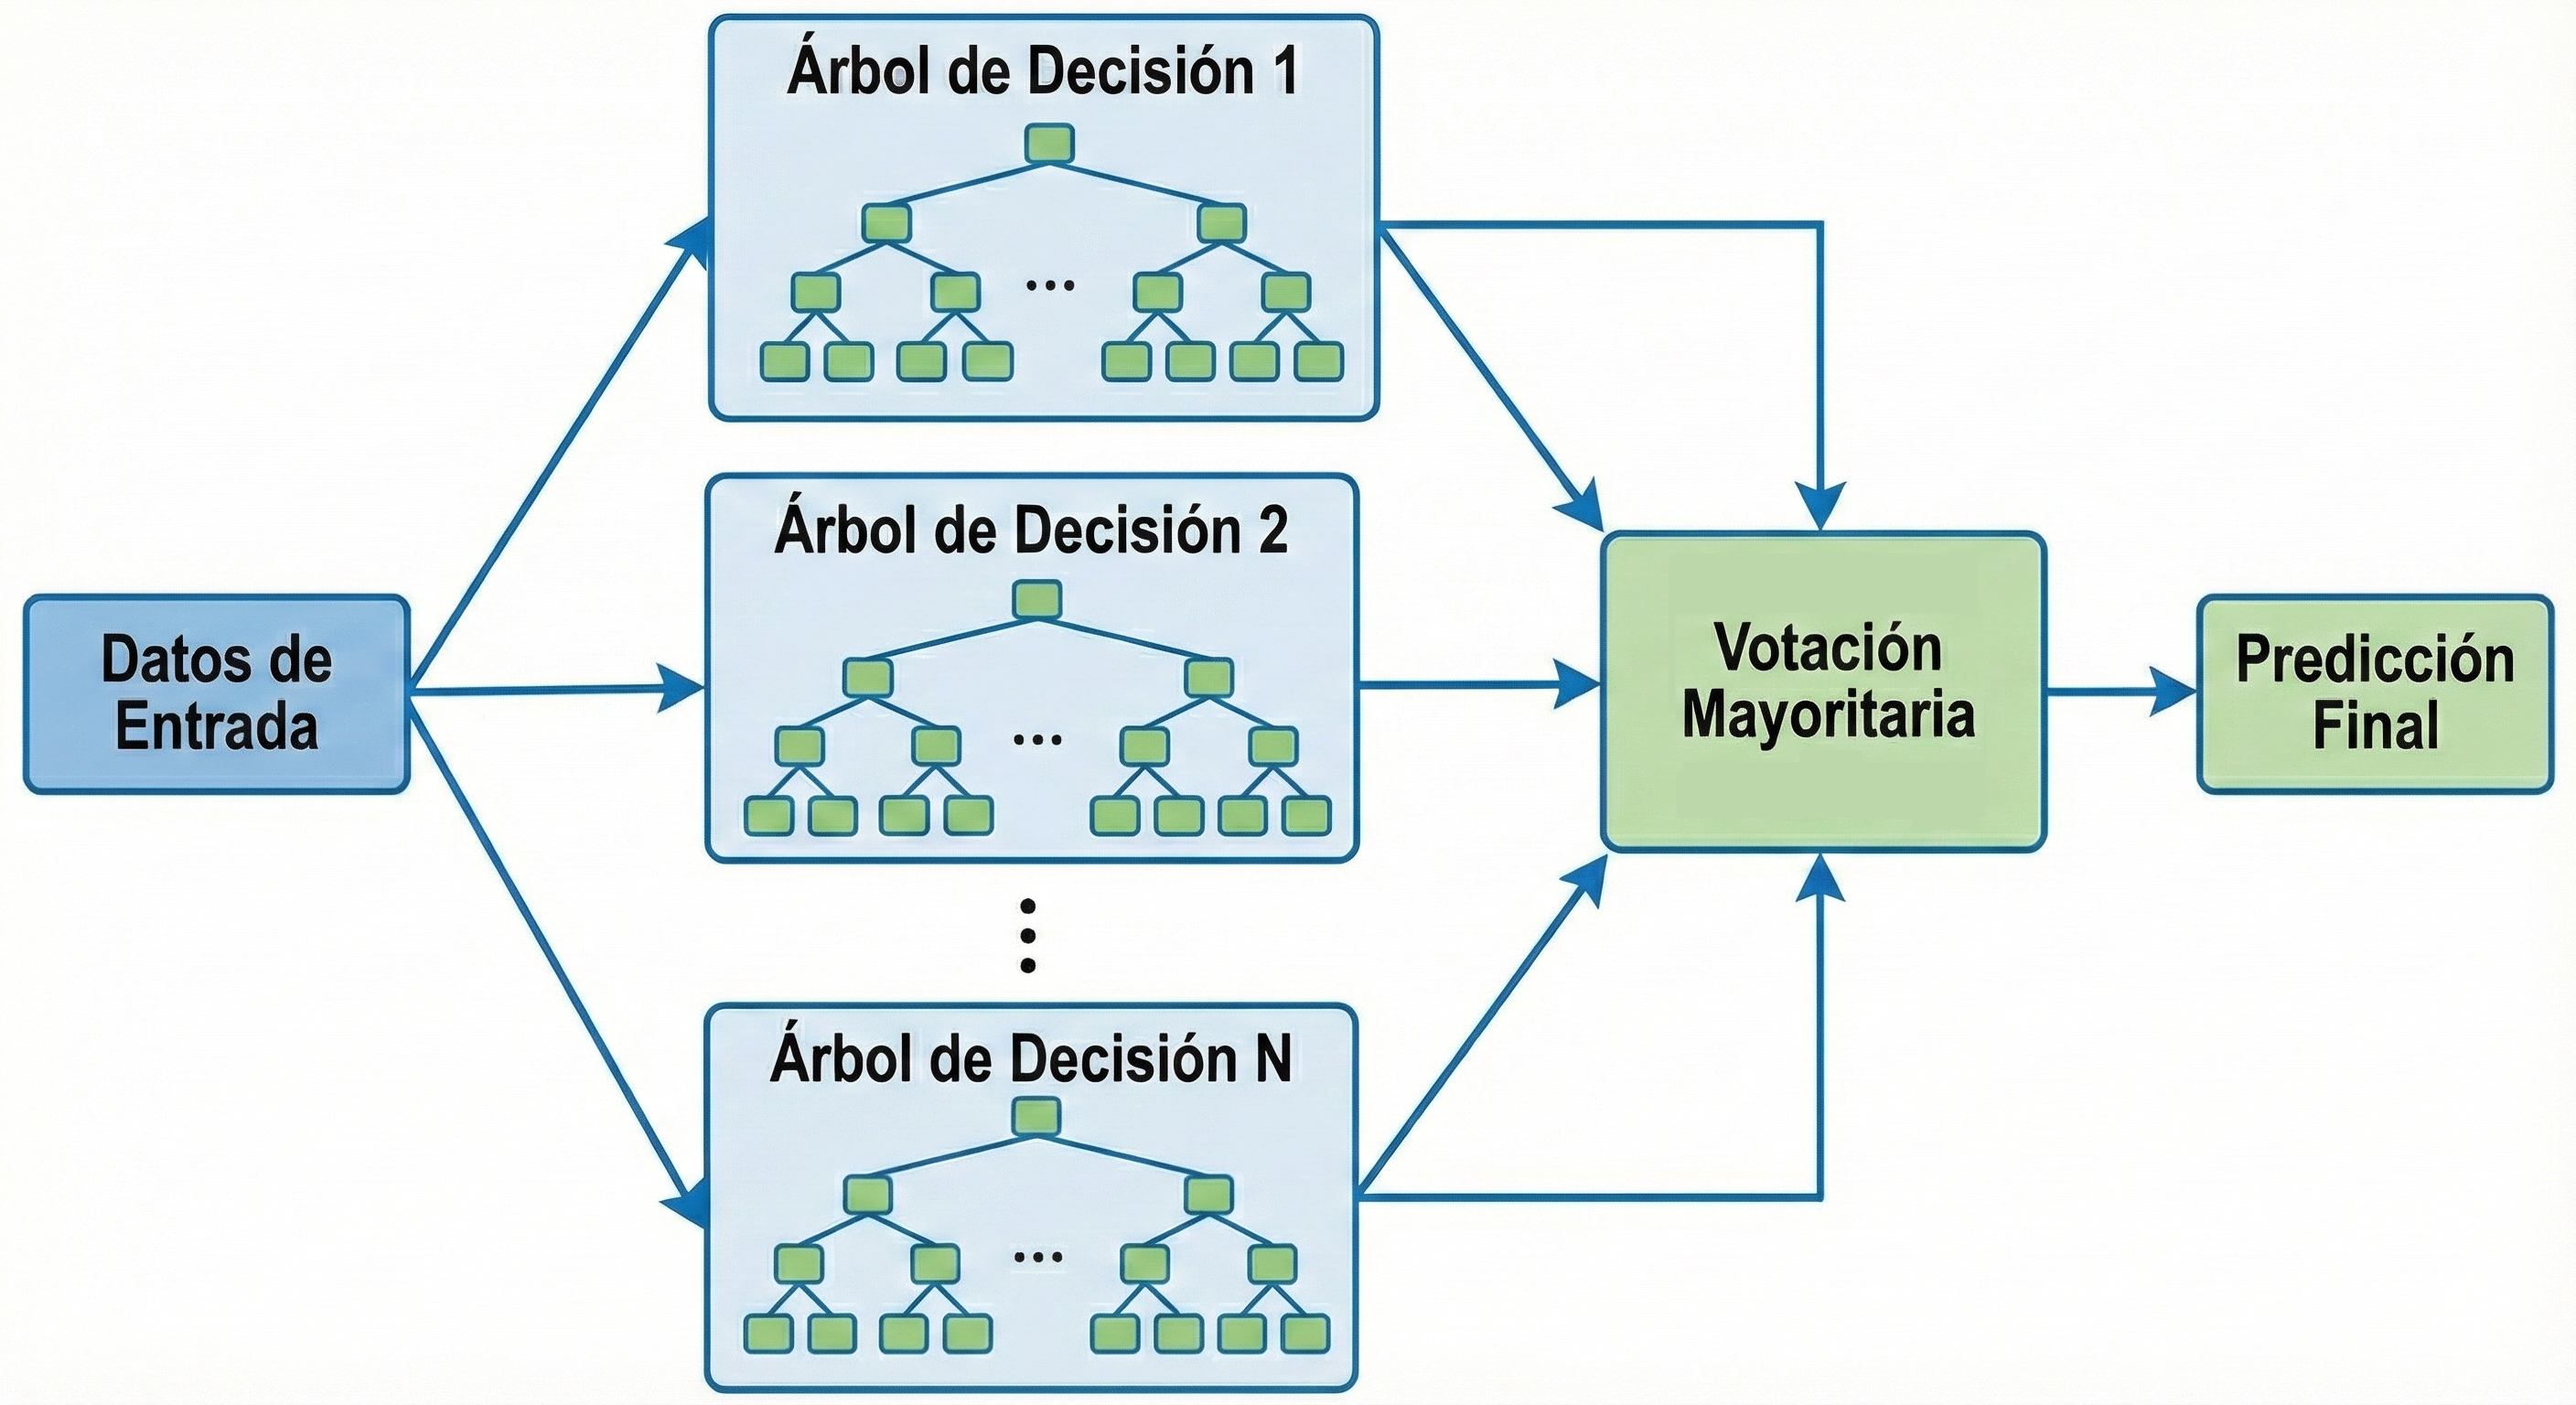
\includegraphics[width=0.9\textwidth]{Imagenes/rf_architecture.png}
	\caption{Arquitectura del clasificador Random Forest. El diagrama ilustra el mecanismo de ensamble: múltiples árboles de decisión ($Tree_1 \dots Tree_n$) procesan la entrada independientemente. La clase final se determina mediante la mayoría de votos (Majority Voting), lo que reduce la varianza y mejora la generalización del modelo.}
	\label{fig:rf_architecture}
\end{figure}

Como se ilustra en la Figura \ref{fig:rf_architecture}, esta estrategia de doble aleatorización reduce significativamente la correlación entre los árboles individuales y mitiga eficazmente el riesgo de sobreajuste (\textit{overfitting}), resultando en un modelo con una alta capacidad de generalización. Adicionalmente, Random Forest proporciona estimaciones automáticas de la importancia de cada característica, lo cual es valioso para interpretar qué aspectos de los movimientos oculares son más discriminativos para la identificación de individuos.